%% $RCSfile: proj_proposal.tex,v $
%% $Revision: 1.2 $
%% $Date: 2010/04/23 02:40:16 $
%% $Author: kevin $

\documentclass[11pt, a4paper, oneside, openright]{article}

\usepackage{float} % lets you have non-floating floats
\usepackage{url} % for typesetting urls
\usepackage{graphicx} % for including images
\usepackage{caption}
\usepackage{program}
\usepackage{tabularx}
\usepackage{colortbl}
\usepackage{hhline}
\usepackage{subcaption}
\newfloat{fig}{thp}{lof}[section]
\floatname{fig}{Figure}


\title{COMP422 Project 2 Report}
\author{Boxiong Tan}

\usepackage[font,ecs]{vuwproject}

% Unless you've used the bschonscomp or mcompsci
%  options above use
   \otherdegree{COMP422 --- Data Mining, Neural Networks and Genetic Programming}
% here to specify degree

% Comment this out if you want the date printed.
%\date{}

\begin{document}

% Make the page numbering roman, until after the contents, etc.
\frontmatter

%%%%%%%%%%%%%%%%%%%%%%%%%%%%%%%%%%%%%%%%%%%%%%%%%%%%%%%

\begin{abstract}
This report contains six questions. The first is using multilayer
feedforward neural network and genetic programming to solve XOR problem. Then make a comparison between
these two approaches. The second question related to digit recognition using neural networks and nearest neighbour method. The third question, symbolic regression problem is a classic problem for genetic programming. The fourth question shows that GP also can be a classifier. The fifth question use GP method as a feature construction method. In question six, we apply two feature selection approaches: wrapper and filter. Then we make a comparison between these two approaches.
\end{abstract}

%%%%%%%%%%%%%%%%%%%%%%%%%%%%%%%%%%%%%%%%%%%%%%%%%%%%%%%

\maketitle

%\tableofcontents

% we want a list of the figures we defined
%\listof{fig}{Figures}

%%%%%%%%%%%%%%%%%%%%%%%%%%%%%%%%%%%%%%%%%%%%%%%%%%%%%%%

\mainmatter

%%%%%%%%%%%%%%%%%%%%%%%%%%%%%%%%%%%%%%%%%%%%%%%%%%%%%%%

\section{Tools and Environment:}
Operating System: Unix/Linux
\newline Programming Language: Python, Shell
\newline Tools and Libraries: SNNS, Weka, Deap\cite{DEAP_JMLR2012}

\section{XOR Problem:}
\subsection{GP Approach}
Genetic programming is a special field of evolutionary computation that aims at building programs automatically to solve problems independently of their domain. Although there exists diverse representations used to evolve programs, the most common is the syntax tree.
\subsection{Function set and terminal set}
In the function set, the three logical operators were used to form the function set:
\newline \hspace*{5cm} $FuncSet = \{\wedge, \vee, \lnot\}$
\newline The $\wedge, \vee, \lnot$ operators have their usual meanings. $\wedge$ and $\vee$ take two arguments. 
The terminal set contains constants and the arguments. In this case, the constants only contain boolean values: $True$ and $False$.
 \newline \hspace*{5cm} $TermSet = \{True, False, Input1, Input2\}$
\subsection{Fitness Function}
The fitness function uses the truth table of XOR to validate the genetic programs. The truth table contains four data sets:
  \begin{figure}[!ht]
  \centerline{\fbox{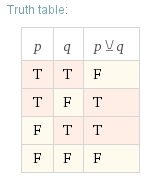
\includegraphics[scale=0.9]{./pics/TruthTable.png}}}
  \caption{XOR truth table}
  \label{fig:xortruth}
  \end{figure}
\newline If the genetic program successfully calculate the value, the fitness will increase by one. 

\begin{program}
\mbox{pseudocode:}
\hspace *{4cm} \IF genetic\_program\_func(input1, input2) == desired\_value:
 \\%
	\hspace*{5mm} fitness = fitness + 1
\end{program}
The range of the fitness value is from 0 to 4. Clearly, when fitness equals 4, the genetic program calculates four dataset correctly.

\subsection{Parameters}
In order to conclude what influence it may has in terms of different parameters each. We made 5 GP programs with one different parameter. Therefore we could see how the different parameters impact on GP.

There  are 4 different parameters: crossover rate, mutation rate, max mutation tree size and population.
\begin{table}[H]
\centering
\begin{tabular}{|l|l|l|l|l|l|}
\hline
\multicolumn{1}{|c|}{\textbf{}} & \multicolumn{1}{c|}{\textbf{Default}} & \multicolumn{1}{c|}{\textbf{Larger POP}} &\multicolumn{1}{c|}{\textbf{Larger CR}} &\multicolumn{1}{c|}{\textbf{Larger MR}} &\multicolumn{1}{c|}{\textbf{Larger MT}}\\
\hline
population(POP)    &20     &40        &20    &20 &20                    \\
\hline
Crossover rate(CR)    &0.6  &0.6   &0.8   &0.6 &0.6                   \\
\hline
Mutation rate(MR)  &0.02  &0.02  &0.02  &0.1 &0.02              \\
\hline
Max mutation tree size(MT)    &4  &4 &4  &4 &6                     \\
\hline
\end{tabular}
\end{table}
We would employ a box plot chart to visualize the final result which will be shown in the result analysis section.

\subsection{Termination criteria}
Once the fitness value equals four, the GP program stopped and returns the result. 
\subsection{Result Analysis}
Three best genetic program for XOR problem:
\begin{enumerate}
\item $((x \vee x) \vee (y \vee x)) \wedge  \lnot(y \wedge x)))$
\item $(y \vee x) \wedge \lnot(y \wedge x)$
\item $((x \vee y) \vee x)  \wedge \lnot(x \wedge y)$
\end{enumerate}

As we discussed in the previous section,  we  test 5 groups of GP using different parameters. Then we use a box plot  chart to visualize the result.

  \begin{figure}[!ht]
  \centerline{\fbox{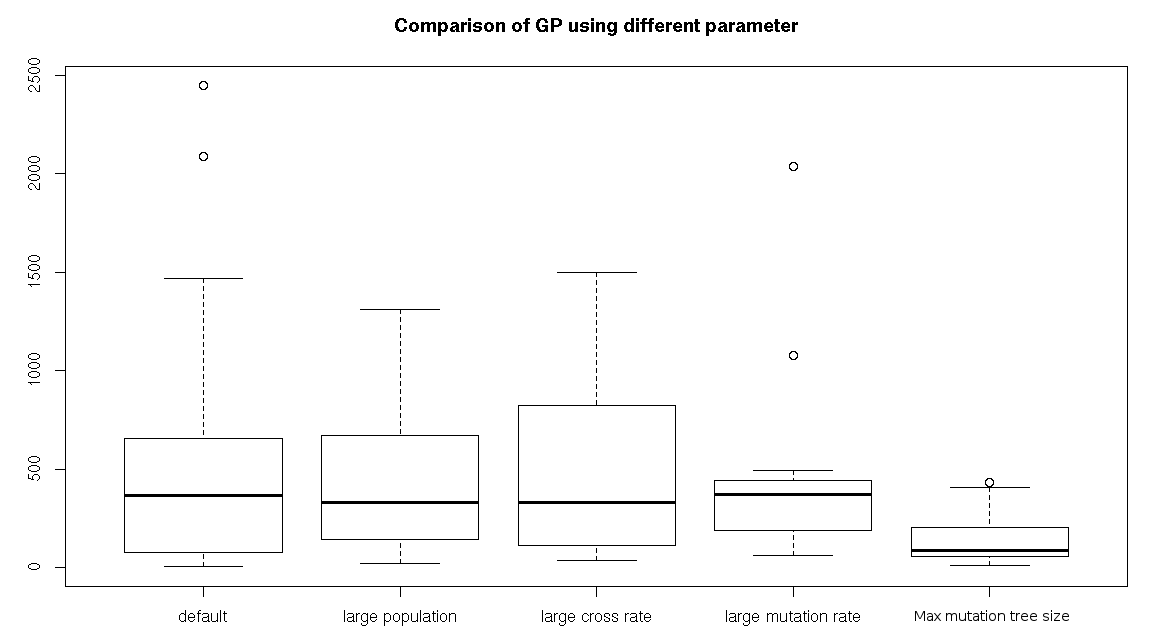
\includegraphics[scale=0.55]{pics/boxplot.png}}}
  \caption{comparison of GP using different parameter}
  \label{fig:comparison}
  \end{figure}

As we can see from Figure \ref{fig:comparison}, the y axis shows the number of generations. The x axis shows the categories of GP. Figure \ref{fig:comparison} shows that the larger mutation tree size (maximum 6 depth) could largely improve the overall performance by significantly reduce the generations. Larger mutation rate also has a significant influence on the result. The overall performance increased, however the median value does not improve at all. Population and larger cross rate have little impact on the result, the reason may because our question is relatively easy and small scale. If we conduct a very complex question that a larger population could have large impact because of the diversity of the gene.


\subsection{Artificial Neural Network Approach}
\subsubsection{One hidden layer, two hidden nodes}
We built a neural network using SNNS \cite{Petron99} with 2 input nodes, 2 hidden nodes and 1 output node.
  \begin{figure}[!ht]
  \centerline{\fbox{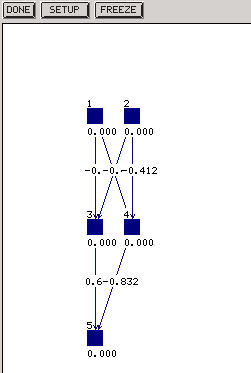
\includegraphics[scale=0.9]{pics/neural.png}}}
  \caption{neural network architecture}
  \label{fig:neural}
  \end{figure}

Then we load the xor problem pattern into SNNS. It  defines the number of class, the number of input nodes, the number of output nodes and each pattern. We initialize the neural network with random weights.  As we can see from Figure \ref{fig:neural}, the neural network are fully connected,  all connections are initialized with random weights.

We use training set to train this neural network with 0.2 learning rate. In the hidden nodes and output nodes, we use sigmoid function as the activate function. We defines 10, 000 epochs as a stopping criteria. Figure 
\ref{fig:errorate} shows the  error rate of  this neural network drops significantly along with training process.
  \begin{figure}[!ht]
  \centerline{\fbox{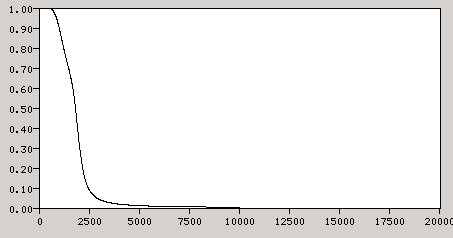
\includegraphics[scale=0.9]{pics/errorate.png}}}
  \caption{error rate drops along with the training process}
  \label{fig:errorate}
  \end{figure}

During the 10,000 epochs training process, the weights of the connections gradually changed. The bias of each hidden nodes and output node also changed. Figure \ref{fig:aftertrain} shows the result of test, using four patterns after 10, 000 epochs training. We could easily see the changes in weights, but the SNNS does not show the bias on the graph. Clearly, the neural network produces a good result by reaching more than 97\% accuracy.

  \begin{figure}[!ht]
  \centerline{\fbox{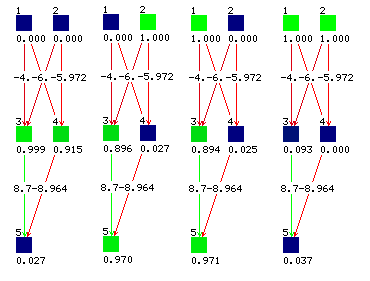
\includegraphics[scale=0.9]{pics/aftertrain.png}}}
  \caption{test with four patterns after 10,000 epochs training}
  \label{fig:aftertrain}
  \end{figure}

\subsubsection{One hidden layer, one hidden node}
As a comparison, we use a different structure neural network to do the classification. Figure \ref{fig:neural_2} shows the  neural network with only one hidden node, however, it has shortcut between input nodes and output node. If we only use one hidden node without any shortcuts. Then the neural network could never solve the XOR problem no matter how many epochs it takes.
  \begin{figure}[!ht]
  \centerline{\fbox{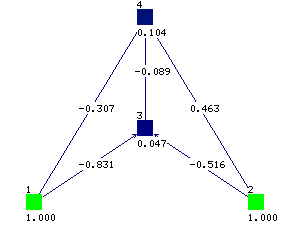
\includegraphics[scale=0.9]{pics/neural_2.png}}}
  \caption{neural network architecture}
  \label{fig:neural_2}
  \end{figure}
\newline We also use four patterns to train the neural network. We train it with 10,000 epochs.We test four patterns. The result shows 96.5\% classification accuracy.

\subsubsection{Comparison between two architecture}
As we use same training pattern, same epochs to train two neural networks, clearly, two hidden nodes could produce better result (97\%). On the other hand, the training process of neural network with one hidden node is faster than 2 hidden nodes neural network. This is because when apply the gradient descent algorithm, clearly there is less computation in the one hidden node neural network.


\subsection{Comparison between Neural network and GP}
Neural network and GP are quite different approaches with different purposes. Neural network is a classifier. However, GP is a searching algorithm. Although approaches could solve the XOR problem, they actually produce complete different solutions. 

Neural network itself is the solution to this problem. Because after certain times of epoch of training, the neural network has the ability to solve this problem.

On the other hand, GP is an algorithm try to search for a solution. After generation and generations, GP could find a solution with ideal accuracy in this case.


\section{Digit Recognition}
This question concerns applying neural networks and nearest neighbour to 4 digit datasets. The dataset that the report chooses: 1( 0\% noise ), 4( 15\% noise), 6( 30\% noise), 9( 60\% noise).

We first clean up the raw datasets. Divide all dataset into training set and test set, each  of set contains 500 lines data.
Then we apply neural network and nearest neighbour using Weka\cite{Hall:2009:WDM:1656274.1656278}.
\subsection{First Dataset with no noise}
Since there is no precise standard of how to choose the number of hidden layer and hidden nodes. What we are trying to do is manually adjust these numbers and see if the neural network produce a good result. We set learning rate = 0.3, momentum = 0.2, Stopping criteria: 500 epochs

We have tried many architectures:
\begin{table}[H]
\centering
\begin{tabular}{|l|l|l|}
\hline
\multicolumn{1}{|c|}{\textbf{hidden layers}} & \multicolumn{1}{c|}{\textbf{hidden nodes}} 
& \multicolumn{1}{c|}{\textbf{Training accuracy}}\\
\hline
1     &1 &30\%                                    \\
\hline
1    &2 &70\%                                  \\
\hline
1   &3 &100\%                                             \\
\hline
2 &each layer 1 node &30\%                                            \\
\hline
2  &each layer 2 nodes &40\%                                              \\
\hline
\end{tabular}
\end{table}
As we can see from the above table, more layers does not necessarily improve the performance. A neural network with 1 hidden layer and 3 hidden nodes could produce a almost perfect result.
Figure \ref{fig:confusion} shows the confusion matrix produced by testing with the test set.
  \begin{figure}[!ht]
  \centerline{\fbox{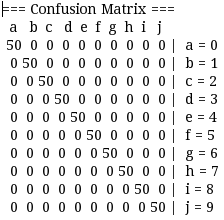
\includegraphics[scale=0.9]{pics/confusion.png}}}
  \caption{confusion matrix}
  \label{fig:confusion}
  \end{figure}
In comparison with KNN.
We employ KNN classifier with 1 neighbour.
The correct rate reach 100\% with 0 second.
In comparison with 3 hidden nodes neural network. The training process took neural network 6.2 seconds. Clearly, KNN performance better in this task.

\subsection{Fourth Dataset with 15\% noise}
We set:  learning rate = 0.3, momentum = 0.2, Stopping criteria: 500 epochs
\begin{table}[H]
\centering
\begin{tabular}{|l|l|l|}
\hline
\multicolumn{1}{|c|}{\textbf{hidden layers}} & \multicolumn{1}{c|}{\textbf{hidden nodes}} 
& \multicolumn{1}{c|}{\textbf{Training accuracy}}\\
\hline
1     &3 &91.4\%                                    \\
\hline
1    &4 &99\%                                  \\
\hline
1   &5 &99.2\%                                             \\
\hline
2 &first layer 3,second layer 2  &58.2\%                                            \\
\hline
2  &each layer 3 nodes &69.8\%                                              \\
\hline
\end{tabular}
\end{table}

Since 3 hidden nodes in one hidden layer work well in no noise dataset, we apply this in 15\% noise dataset. The result shows 91.4\% accuracy. Then we try 4 and 5 hidden nodes, they both improved hugely in the performance. Then we try multi-hidden layers, as a result, it does not work well.
Figure \ref{fig:confusion_2} is the confusion matrix, produced by 5 hidden nodes neural network tested on testing set.
  \begin{figure}[!ht]
  \centerline{\fbox{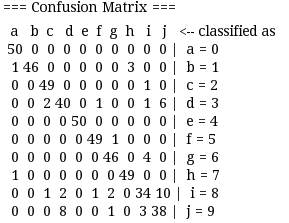
\includegraphics[scale=0.9]{pics/confusion_2.png}}}
  \caption{confusion matrix}
  \label{fig:confusion_2}
  \end{figure}
\newline In comparison with KNN:
KNN achieve 93.4\% accuracy with 0 second learning time.
In comparison with the best result in neural network, 5 hidden nodes in one hidden layer. It took neural network 4.62 seconds to train and 4.5 seconds to test. It achieve 90.2\% accuracy in the testing set. The KNN achieve much better performance.

\subsection{Sixth Dataset with 30\% noise}
We set:  learning rate = 0.3, momentum = 0.2, Stopping criteria: 500 epochs
\begin{table}[H]
\centering
\begin{tabular}{|l|l|l|}
\hline
\multicolumn{1}{|c|}{\textbf{hidden layers}} & \multicolumn{1}{c|}{\textbf{hidden nodes}} 
& \multicolumn{1}{c|}{\textbf{Training accuracy}}\\
\hline
1     &6 &97.4\%                                    \\
\hline
1    &7 &99\%                                  \\
\hline
1   &8 &99\%                                             \\
\hline
2 &each layer 4 nodes  &89.2\%                                            \\
\hline
2  &each layer 5 nodes &95.8\%                                              \\
\hline
2  &each layer 8 nodes &99.4\%                                              \\
\hline
\end{tabular}
\end{table}

As we can see, 7 and 8 hidden nodes both achieve 99\% training accuracy. In terms of time consuming, 7 nodes performance better. Furthermore, 2 hidden layers with 8 nodes in each could achieve 99.4\% training accuracy.
When we test the neural network with 2 hidden layers and 16 hidden nodes, it could  only achieve 78.6\% accuracy.
  \begin{figure}[!ht]
  \centerline{\fbox{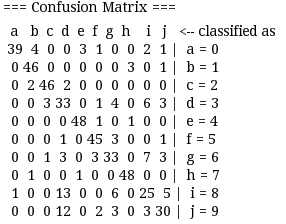
\includegraphics[scale=0.9]{pics/confusion_3.png}}}
  \caption{confusion matrix}
  \label{fig:confusion_3}
  \end{figure}
In comparison with KNN, the KNN also achieve 78.6\% accuracy in the test set. In terms of time consuming, the KNN performs better.

\subsection{Fourth Dataset with 60\% noise}
We set:  learning rate = 0.3, momentum = 0.2, Stopping criteria: 500 epochs
\begin{table}[H]
\centering
\begin{tabular}{|l|l|l|}
\hline
\multicolumn{1}{|c|}{\textbf{hidden layers}} & \multicolumn{1}{c|}{\textbf{hidden nodes}} 
& \multicolumn{1}{c|}{\textbf{Training accuracy}}\\
\hline
1     &10 &92.6\%                                    \\
\hline
1    &15 &97\%                                  \\
\hline
1   &20 &96.8\%                                             \\
\hline
1   &50 &97.4\%                                             \\
\hline
2 &each layer 5 nodes  &73.6\%                                            \\
\hline
2  &each layer 10 nodes &94.4\%                                              \\
\hline
2  &each layer 15 nodes &96.6\%                                              \\
\hline
3 &each layer 15 nodes &97.6\%                                              \\
\hline
\end{tabular}
\end{table}

With 3 hidden layers and 15 nodes in each hidden layer, the neural network could reach a decent result. However, when apply it to the test set. The classification accuracy drop to 47.6\%. On the other hand, one hidden layer with 15 nodes could get 54\% accuracy. In comparison with KNN, the KNN could only achieve 43.6\% accuracy. The neural network have better denoising ability.

\section{Symbolic Regression Problem}
Symbolic regression is one of the best known problems in GP\cite{koza1992genetic}. Symbolic regression is a type of regression analysis that searches the space of mathematical expressions to find the model that best fits a given dataset, both in terms of accuracy and simplicity.

\subsection{Function set and terminal set}
In the function set, the 6 operators were used to form the function set:
\newline \hspace*{4cm} $FuncSet = \{+, -, \times, \div, cos, sin\}$
\newline The terminal set contains constants and the arguments. In this case, the constants are numerics value from 0 to 9. 

Since this given function is a piecewise function:
  \begin{figure}[!ht]
  \centerline{\fbox{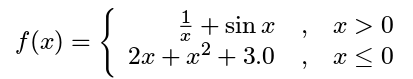
\includegraphics[scale=0.9]{pics/formula.png}}}
  \caption{Target formula}
  \label{fig:formula}
  \end{figure}

In terms of simplicity, we only choose to search for the best solution range from (-5, 5).
  \begin{figure}[!ht]
	\centering
	\begin{subfigure}[b]{0.4\textwidth}
		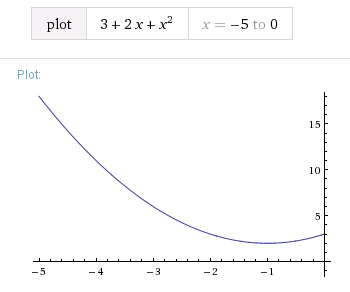
\includegraphics[scale=0.5]{pics/negative.png}
  		\caption{ $3 + 2  \times x + x^2 \in (-5,0]$ }
 		 \label{fig:negative}
	\end{subfigure}
	\begin{subfigure}[b]{0.4\textwidth}
  		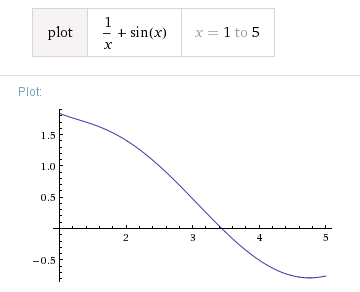
\includegraphics[scale=0.5]{pics/positive.png}
 		 \caption{ $\frac{1}{x} + \sin(x) \in $ (0, 5] }
 	 	\label{fig:positve}
	\end{subfigure}
  \end{figure}

\subsection{Parameters}
In this problem, we use population = 40, cross rate = 0.6, mutation rate = 0.1
\subsection{Fitness Function}
We use the accuracy as the fitness value. The ideal fitness should be 0 or close to 0.
\begin{program}
\mbox{pseudocode:}
\hspace *{4cm} \FOR \hspace*{2mm} from \hspace*{2mm}-5\hspace*{2mm} to\hspace*{2mm} 5:
		sum = sum + (genetic\_program\_func(i)  - desired\_value)
		fitness = sum / 10
 \\%
	fitness =  fitness + 1
\end{program}
The more the fitness close to 0, the better the result it is.
\subsection{Termination criteria}
There are two ways to decide when to stop.
First one is we manually decide how many generation to run. The second choice is we set a threshold of the fitness, when the fitness reach that threshold, it stops.

\subsection{Result Analysis}
As the more accuracy the GP generated, the larger the formula it will be. 
This is genetic program using 150 generations:
\newline \hspace * {5cm} $(x + ((x - 3) \times x))$
\newline After 200 generations, although the fitness become more and more small, the genetic program become human unreadable. Figure \ref{fig:generations} shows the fitness drops along with the generations. Although there is a huge improve 
in the 80 generations, the algorithm does not choose the best instances. If we apply elitism in GP the problem will be solved.
  \begin{figure}[!ht]
  \centerline{\fbox{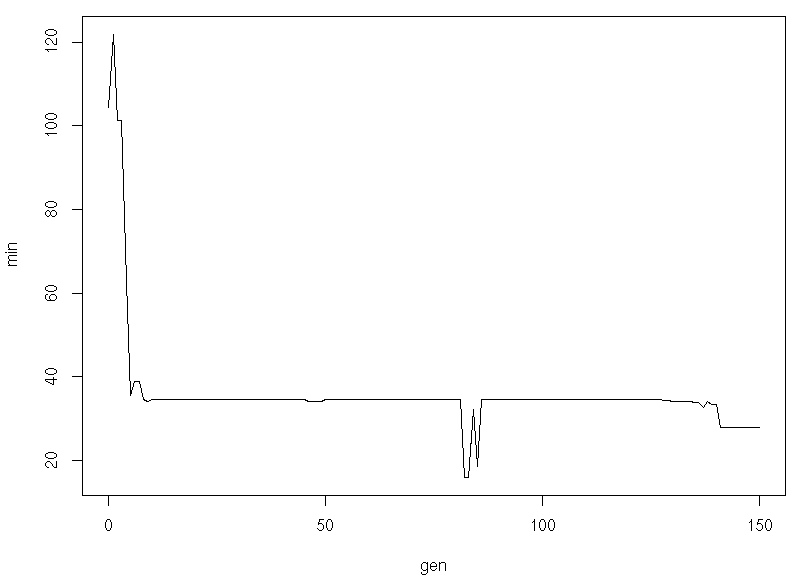
\includegraphics[scale=0.4]{pics/generations.png}}}
  \caption{ the fitness drops along with generations}
  \label{fig:generations}
  \end{figure}
 

\section{Digit Recognition}
The  question is using genetic programming to automatically find out a genetic program to solve the binary classification problem.
\subsection{Primitive set and terminal set}
For this problem, the program uses a primitive set contains six operations:
\newline \hspace*{5cm} $FuncSet = \{+, -, \times, \div, absolute, square\}$
\newline The terminal set contains constants and the arguments. In this case, the constants are numerics value from 0 to 9. 
There are two dataset: liver and pima. Each of the two dataset contains different features. Liver dataset contains 6 features and pima dataset contains 8 features.We use each of the feature as our input parameter.
\newline \hspace*{5cm} $TermSet = \{Features, 0..9\}$
\subsection{Parameters}
In this problem, we use population = 30, cross rate = 0.6, mutation rate = 0.1
\subsection{Fitness Function}
First calculate the result with all input parameters, if the result is greater than 0, then judge  if the desired class is 1, if it is true, then the fitness add 1 over the length of the dataset.
\begin{program}
\mbox{pseudocode:}
\hspace *{3cm} predict\_value = genetic\_program(parameters)
\hspace *{3cm}		Loop \hspace *{2mm}the \hspace *{2mm}whole \hspace *{2mm}dataset:
\hspace *{3cm}			\IF predict\_classes > 0 \hspace *{2mm} \wedge \hspace *{2mm}desired\_class == 1:
							fitness = fitness + 1 / (size\hspace *{2mm} of \hspace *{2mm}the\hspace *{2mm} dataset)
					\ELSE \IF predict\_class <= 0 \hspace *{2mm}\wedge \hspace *{2mm} desired\_class == 0:
					fitness = fitness + 1 / (size \hspace *{2mm}of \hspace *{2mm}the \hspace *{2mm}dataset)			
 \\%
\end{program}
Eventually, the fitness will show the percentage of accuracy classification.
\subsection{Termination criteria}
There are two ways to stop the GP, one is manually set a stopping criteria, for example, the process will stop if it reaches 200 generations. The other way is set an accuracy threshold, for example, if the genetic program could reach 90\% accuracy, then the process stopped.
\subsection{Result Analysis}
After testing for many round, the genetic program could easily reach 70\% accuracy on both datasets but so far the best one could only reach 75\% accuracy.

The report did 15 times running on each dataset,  the mean accuracy of liver dataset is 67\%, the standard deviation is 0.037.          
For the other dataset, pima, the mean accuracy is 70.08\%, and the standard deviation is 0.035.


During the testing, we found sometimes the genetic program could be complete composite by instances. Namely, there is no feature participate in the genetic program.  The reason might be the instances in the dataset is uneven. In order to eliminate any influence that comes from the uneven number of instances, we randomly delete some of the instances to make it even. Then we repeat the experiment. Interestingly, the accuracy drops in both dataset.

\section{Feature Construction}
Feature construction methods may be applied to pursue two distinct goals: reducing data dimensionality and improving prediction performance. In this question, we apply feature construction method using genetic programming(GP). In this report, it mainly focus on reducing data dimensionality. We apply this strategy on two dataset: wine and balance.


In the feature construction paradigm, GP is used to derive a new feature set from the original one. Individuals are often tree like representations of features, the fitness function is usually based on the prediction performance of the classifier trained on these features while the operators can be applications specific. The method essentially performs a search in the new feature space and helps generate a high performance subset of features. The newly generated features may often be more comprehensible and intuitive than the original feature set, which makes GP-related methods well-suited for such tasks.

\subsection{Fitness function}
We used classification accuracy on the training set as the fitness function.  We first use genetic program to calculate all the objects in the wine or balance dataset and generate a file which contrains one new feature. Then, we use this new feature to train naive bayes classifier or decision tree classifier with 10 fold cross-validation.  The classification accuracy is the number of object that are correctly classified by the classifier as a proportion of the total number of object in the training set.

\subsection{Result Analysis}
First, we apply naive bayes classifier and GP feature construction on wine dataset.
The parameter values used in this approach are shown in Table \ref{tab:Parameters}. 
\begin{table}[H]
\centering
\captionof{table}{}
\begin{tabular}{|l|l|}
\hline
\multicolumn{1}{|c|}{\textbf{Parameter}} & \multicolumn{1}{c|}{\textbf{value}} \\
\hline
Population &30 \%                                    \\
Crossover rate    &0.6\%                                  \\
Mutation rate   &0.1\%                                             \\
Max Depth   &20\%                                             \\
\hline
\end{tabular}
\label{tab:Parameters}
\end{table}

These values are determined based on empirical search. In this approach, the learning/evolutionary process is terminated when one of the following conditions are met:
\newline 1. The accuracy is higher than 95\%.
\newline 2. The number of generations reaches the pre-defined number, max\_generations.
The best performance genetic program(lisp program):
\newline \hspace * {4cm} $(- ( \times (f6,  \div (1, f10)),  \div ( \div ( \div (1, f10), f10), f10)))$
  \begin{figure}[!ht]
  \centerline{\fbox{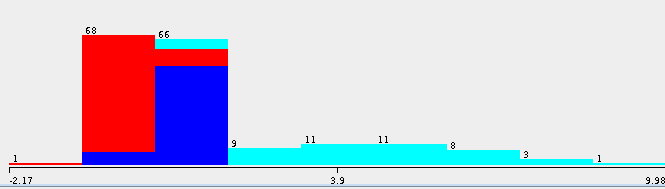
\includegraphics[scale=0.8]{pics/classes.png}}}
  \caption{new feature separate three classes}
  \label{fig:classes}
  \end{figure}
\newline We could easily see from figure \ref{fig:classes}. Each color represents a class. The new feature successfully separate the classes in the dataset, although there exists overlapping.

Then, we test the performance of this new feature with Weka.
The results are shown below:
\\
\newline Correctly Classified Instances   \hspace * {4mm}      156     \hspace * {4mm}           87.6404 \%
\newline Incorrectly Classified Instances   \hspace * {4mm}      22     \hspace * {4mm}           12.3596 \%
\\
\\
As can be seen from the result, the new feature achieve 87.6\% accuracy on classification. The accuracy is reasonably good especially consider the number of feature has been reduced from 13 to 1.
\\
\\
Then we compare the result with using all features.
\\
\newline Correctly Classified Instances   \hspace * {4mm}      172    \hspace * {4mm}           96.6292 \%
\newline Incorrectly Classified Instances   \hspace * {4mm}      6     \hspace * {4mm}           3.3708 \%
\\
\newline Clearly, the result shows there are still advantages using all features. The accuracy is still higher than the construction feature.

We apply the same strategy on balance dataset.
The best performance genetic program:
\newline \hspace * {2.5cm} $+(\div ( \div (f0, f3), \div( \div (f2, f3), \div (f1, f3))), \div ( \div (f0, f2), \div (f0, f2)))$
\newline Then we use the produced feature dataset to do the classification, the result shows below:
\\
\newline Correctly Classified Instances      \hspace * {4mm}   613      \hspace * {4mm}         98.08   \%
\newline Incorrectly Classified Instances  \hspace * {4mm}      12       \hspace * {4mm}         1.92   \%
\\
\\
Surprisingly, the construction feature produce a fairly good result.
The figure \ref{fig:classes_2} shows the classification of three classes using the new feature:

  \begin{figure}[!ht]
  \centerline{\fbox{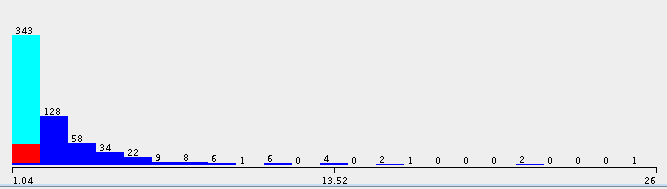
\includegraphics[scale=0.8]{pics/classes_2.png}}}
  \caption{new feature separate three classes}
  \label{fig:classes_2}
  \end{figure}

Then we compare this result with using all features.
\\
\newline Correctly Classified Instances   \hspace * {4mm}      565    \hspace * {4mm}           90.4    \%
\newline Incorrectly Classified Instances  \hspace * {4mm}      60     \hspace * {4mm}           9.6    \%
\\
  \begin{figure}[!ht]
  \centerline{\fbox{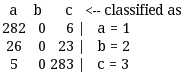
\includegraphics[scale=1]{pics/matrix.png}}}
  \caption{confusion matrix}
  \label{fig:matrix}
  \end{figure}
\newline The result(Figure \ref{fig:matrix}) shows that no class b object was correctly classified using all the features. On the other hand, the construction feature could successfully classify all the class b object. In terms of overall performance, the construction feature is also much better than using all features.  

\section{Feature Selection}
In this question, this report chooses two single feature ranking algorithms (Information Gain(IG) and Chi-square) and apply them to Wisconsin Breast Cancer and Sonar data sets. Then the report gives two comparison, one is compare the performance of the classifier using all the features with N top features.The other one is comparison between  filter approach and wrapper approach.

\subsection{Information Gain and Chi-square ranking algorithm}
In this question,we would use Weka to solve our problem.
First, we apply information gain ranking algorithm, then we apply naive bayes to do the classification.

We apply IG on sonar dataset.
Search Method:
	Attribute ranking.
Attribute Evaluator (supervised, Class (nominal): 61 classes):
Information Gain Ranking Filter

\begin{table}[H]
\centering
\begin{tabular}{|l|l|}
\hline
\multicolumn{1}{|c|}{\textbf{Ranked}} & \multicolumn{1}{c|}{\textbf{Feature}} \\
\hline
0.2014    &f11                                     \\
\hline
0.1779    &f12                                \\
\hline
0.1498  &f9                                             \\
\hline
0.143   &f10                                             \\
\hline
0.1208   &f13                                             \\
\hline
\end{tabular}
\end{table}


As a result,  the top 5 features are 9, 10, 11, 12, 13. Then we apply these 5 features in classification. The table below shows the result:
\\
\newline Correctly Classified Instances      \hspace * {4mm}   146       \hspace * {4mm}        70.1923 \%
\newline Incorrectly Classified Instances    \hspace * {4mm}    62   \hspace * {4mm}            29.8077 \%
\\
\\
We then use Chi-square ranking algorithm to select features. Interestingly, the Chi-square choose the exact same top 5 features: f11, ,f12 ,f9,f10,f13.

As a comparison, we apply all 60 features on sonar dataset:
We also use naive bayes in this task:
\\
\newline Correctly Classified Instances     \hspace * {4mm}    152      \hspace * {4mm}         73.0769 \%
\newline Incorrectly Classified Instances   \hspace * {4mm}     56       \hspace * {4mm}        26.9231 \%
\\
\\
The result shows that there is still some advantages in using all features especially the dataset or the number of feature is relatively small.

We apply information gain on wbcd dataset:
Information Gain Ranking Filter

\begin{table}[H]
\centering
\begin{tabular}{|l|l|}
\hline
\multicolumn{1}{|c|}{\textbf{Ranked}} & \multicolumn{1}{c|}{\textbf{Feature}} \\
\hline
0.685    &f23                                     \\
\hline
0.6686    &f24                                \\
\hline
0.6665  &21                                             \\
\hline
0.6478   &f28                                             \\
\hline
0.6347   &f8                                            \\
\hline
\end{tabular}
\end{table}

Then we use these 5 features in classification.
The result shows:
\\
\newline Correctly Classified Instances    \hspace * {4mm}     538    \hspace * {4mm}           94.5518 \%
\newline Incorrectly Classified Instances  \hspace * {4mm}      31     \hspace * {4mm}           5.4482 \%
\\
\\
Then we use Chi-square to do the ranking, as the same with the previous dataset, we got the same selection of features:, f8, f21, f23, f24, f28


In comparison, we use all 30 features:
\\
\newline Correctly Classified Instances    \hspace * {4mm}     534      \hspace * {4mm}         93.8489 \%
\newline Incorrectly Classified Instances   \hspace * {4mm}     35       \hspace * {4mm}         6.1511 \%
\\
\\
The top features could approvide a better result than using all features. It is not only efficient but also effective.

\subsection{Comparison between wrapper and filter approaches}
First we apply wrapper approach on sonar dataset using BestFirst as our search method.
The result shows that there are 5 features get selected:12,17,18,24,39.
Then we apply these 5 features in classification:
\\
\newline Correctly Classified Instances     \hspace * {4mm}    160    \hspace * {4mm}           76.9231 \%
\newline Incorrectly Classified Instances   \hspace * {4mm}     48      \hspace * {4mm}         23.0769 \%
\\
\\
As the result shows, using wrapper approach, the accuracy could reach 76.9\%, better than using all 60 features (73\%)  and the Information Gain top 5 features (70.2\%). The reason probably because the wrapper approach tries all possible subset of features and select the best performance combination. However, the filter approach only treat each attribute as independent feature and test on each attribute individually. The result of filter approach might not be so good because some of these selected features are redundant. 


We then test wrapper approach on wbcd dataset.
 The wrapper approach shows that there are 6 features being selected: 12, 15, 19, 22,23,25
Then we use these 6 features on wbcd classification:
\\
\newline Correctly Classified Instances    \hspace * {4mm}     553    \hspace * {4mm}           97.188  \%
\newline Incorrectly Classified Instances  \hspace * {4mm}      16     \hspace * {4mm}           2.812  \%
\\
\\
The result shows the features selected by wrapper approach could reach a better result, compare with using all 30 features(93.8\%) and use information gain 5 top ranking features(94.6\%).

\subsection{Conclusions}
Although using the wrapper approach could get slightly better result, in terms of efficient and effective, the wrapper approach might not be the best choice because of the extra computation. In practice, to choose which approach in use still depend on the question, if the question is not urgent or require high accuracy, the information gain top features could be a good choice. However, some task like diseases classification which require high level accuracy, the wrapper approach is more suitable.
%%%%%%%%%%%%%%%%%%%%%%%%%%%%%%%%%%%%%%%%%%%%%%%%%%%%%%%
\backmatter
%%%%%%%%%%%%%%%%%%%%%%%%%%%%%%%%%%%%%%%%%%%%%%%%%%%%%%%

%\bibliographystyle{ieeetr}
\bibliographystyle{acm}
\bibliography{report}
\end{document}
